% Screw-axis concept diagram for notebook 01 (Rigid-Body Motions).
% Standalone document: compiles on its own with `lualatex screw_axis.tex`,
% and is loaded by notebooks via _shared/tikz.render_tikz_file(...).
\documentclass[tikz,border=4pt]{standalone}
\usepackage{amsmath}
\usepackage{tikz}
\usepackage{pgfplots}
\pgfplotsset{compat=1.18}
\usetikzlibrary{arrows.meta,calc,3d,angles,quotes,decorations.markings}
\begin{document}
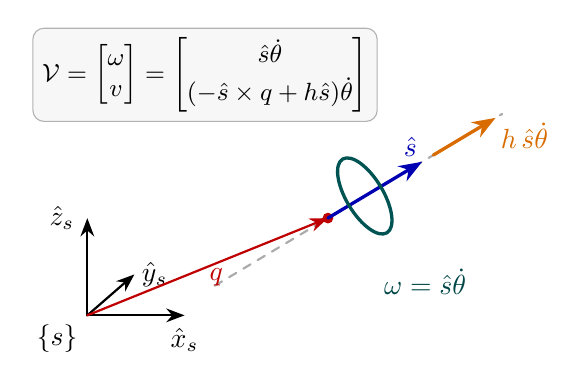
\begin{tikzpicture}[>=Stealth,scale=1.3,line cap=round,line join=round]
  % --- space frame {s} ---
  \draw[->,thick] (0,0) -- (0.95,0) node[below=1pt]{$\hat{x}_s$};
  \draw[->,thick] (0,0) -- (0,0.95) node[left=1pt]{$\hat{z}_s$};
  \draw[->,thick] (0,0) -- (0.46,0.40) node[right=-1pt]{$\hat{y}_s$};
  \node[below left] at (0,0) {$\{s\}$};

  % --- screw axis: a point Q on it, axis direction s-hat (q is NOT parallel to axis) ---
  \coordinate (Q)    at (2.35,0.95);
  \coordinate (sdir) at (0.92,0.55);
  \draw[dashed,gray!65,thick] ($(Q)-1.2*(sdir)$) -- ($(Q)+1.85*(sdir)$);

  % --- vector q from {s} to the point Q on the axis ---
  \draw[->,thick,red!75!black] (0,0) -- (Q) node[midway,below right=-3pt]{$q$};
  \fill[red!75!black] (Q) circle (1.5pt);

  % --- unit screw direction s-hat along the axis ---
  \draw[->,very thick,blue!70!black] (Q) -- ($(Q)+(sdir)$) node[above left=-2pt]{$\hat{s}$};

  % --- angular velocity omega = s-hat*thetadot : a ring around the axis at Q ---
  \begin{scope}[shift={(Q)},rotate=31]
    \draw[->,very thick,teal!65!black] (0.42,0) ellipse [x radius=0.18, y radius=0.42];
  \end{scope}
  \node[teal!55!black] at ($(Q)+(0.95,-0.62)$) {$\omega=\hat{s}\dot{\theta}$};

  % --- pitch translation h*s-hat*thetadot : along the axis past s-hat ---
  \draw[->,very thick,orange!85!black] ($(Q)+1.12*(sdir)$) -- ($(Q)+1.78*(sdir)$)
        node[below right=-2pt]{$h\,\hat{s}\dot{\theta}$};

  % --- twist definition ---
  \node[align=left,draw=black!30,rounded corners,fill=black!3,font=\small] at (1.15,2.35)
    {$\mathcal{V}=\begin{bmatrix}\omega\\ v\end{bmatrix}
       =\begin{bmatrix}\hat{s}\dot{\theta}\\[2pt]
        (-\hat{s}\times q+h\hat{s})\dot{\theta}\end{bmatrix}$};
\end{tikzpicture}
\end{document}
